\chapter{Component separation: finding the cells}\label{ch:separation}

\section{The problem}

A blood specimen is a mixture. At locus $i$ its methylation is, to good approximation,
\begin{equation}
  \beta_i=\sum_c f_c\,\mu_{ic}+\epsilon_i,\qquad f_c\ge0,\ \ \sum_c f_c\le1,
  \label{eq:mix}
\end{equation}
where $\mu_{ic}$ is cell $c$'s methylation at locus $i$ from the atlas and $f_c$ its fraction of the DNA in the tube. This is the
methylome's component separation, and it is solved by constrained least squares on a set of loci that separate the cells
(markers)~\cite{Houseman2012,Salas2022}. On the sky the same equation has frequencies in place of loci and emission laws in place
of cell profiles.

\section{Two jobs, kept apart}

The chain's rule, in the author's words, is \emph{it doesn't matter the fraction; that is a detection issue}. Deconvolution does two
things and they are kept apart:
\begin{enumerate}
\item it decides \emph{which cells are present}, with an interval on each fraction; a cell the solver does not find is not scored;
\item it supplies the fractions the rest of the chain needs to know what the specimen should look like.
\end{enumerate}
It never supplies a cell's $A$. The cell is read on its own identity loci (Chapter~\ref{ch:identity}).

\section{The solver on atlas v2}

The v2 solver reads only atlas v2: no v1 file, marker panel or name. It chooses markers from the atlas posterior, pairwise between
each cell and its nearest neighbours as well as one-against-all, weights each locus by the atlas's posterior uncertainty, and returns
bootstrap intervals on every fraction. It was pre-registered and tested on 24 arrays of blood mixtures made from purified cells in known
proportions~\cite{Salas2018,Salas2022}.

\begin{center}\small
\begin{tabular}{@{}lrl@{}}\toprule
cell group & mean absolute fraction error & bar $\le0.015$ \\\midrule
CD4 T & 0.024 & failed \\
CD8 T & 0.031 & failed \\
NK & 0.0075 & passed \\
B & 0.013 & --- \\
monocytes & 0.015 & --- \\
neutrophils & 0.015 & --- \\
eosinophils & 0.027 & --- \\
basophils & 0.006 & --- \\\bottomrule
\end{tabular}
\end{center}
\measured{} (PROC-DECONV-V2-01, first run, 74 cells.) The failure had a pattern: CD8 was under-read on 19 of 24 arrays and CD4 over-read on
19. A separability report showed why: 24 of the 74 cells had fewer than 20 loci separating them by 0.20 from their nearest cell, and 16 of those
were parent--child pairs or close subsets, such as bulk CD4 T cells beside their naive and memory subsets. A bulk sorted population is, in
methylation, a mixture of its own subsets, so a solver can trade mass between parent and children without changing the fit.

A second pattern was a leak: arrays that contain no endothelium were assigned vascular endothelium. The atlas's vascular endothelium
profile, from one source, itself decomposed into a blend of other endothelia, adipocytes and blood.

Development then changed two things. A sweep over marker schemes chose a hybrid of pairwise and one-against-all markers, which brought CD4, CD8 and NK
inside the bar on the same 24 mixtures (0.014, 0.012, 0.0087) but still called vascular endothelium present on all 24. Excluding that one profile left
the blood errors where they were (CD4 0.012, CD8 0.012, NK 0.009) and removed the leak: the median non-blood fraction fell from 0.017 to 0.004 and no
non-blood cell was called present. \measured{} Eosinophils (0.041) and neutrophils (0.024) remain outside the bar; the atlas's eosinophil profile matches
its own purified arrays, and the shortfall is not yet explained. \openprob

\section{Which cells a specimen can contain}

A solver asked to explain whole blood with every cell in the atlas will use cells that cannot be there if they help the fit. The first v2 readings
of healthy whole blood found the six bone-marrow progenitor populations absorbing a large share of the mass, starving monocytes and B cells
(Chapter~\ref{ch:firstreadings}). A per-specimen scale term did not remove the effect; removing the progenitors from the candidate set for
circulating blood did, and the composition returned to a normal blood picture. The chain now carries specimen-type candidate sets: circulating
blood without progenitors; bone marrow and sorted cells with them. That is a statement about anatomy, not about people. \measured

\section{The transfer function}

A deconvolver explains away anything that looks like a change in composition. A real change in one cell's methylation at loci shared with another
cell is partly absorbed as a change in fractions, and the residual shrinks. In CMB language this is the pipeline's transfer function: the analysis
filters the signal it is meant to find. It was seen empirically before it had a name, as whole chromosomes' signals depleted after deconvolution.
The chain's answer is to read a cell on its identity loci after deconvolution rather than on the residual, and to measure the transfer on constructed
specimens with known changes (Chapter~\ref{ch:discipline}).

\section{Fraction and $A$}

Diluting a cell into a background moves the mean $\beta$ on its identity loci linearly from what the background reads there to the cell's own value.
On constructed specimens built from the first atlas (26 September 2026):

\begin{center}\small
\begin{tabular}{@{}lrrr@{}}\toprule
cell & $A$ at fraction 0 & $A$ pure & first detected at \\\midrule
colon epithelium & 0.869 & 1.004 & 2~\% \\
breast & 0.905 & 0.994 & 35~\% \\
cortical neurons & 1.065 & 0.986 & 1~\% \\
NK cells & 0.942 & 0.992 & 12~\% \\
GMP & 0.919 & 0.986 & 0.5~\% \\
CD4 T cells & 1.037 & 0.991 & 2~\% \\\bottomrule
\end{tabular}
\end{center}
\measured{} A minor cell's reading on the bulk specimen is therefore partly a reading of everything else. The mixture can be inverted,
\begin{equation}
  \bbar_c^{\,\mathrm{own}}=\frac{\bbar_c^{\,\mathrm{specimen}}-\sum_{c'\ne c}f_{c'}\,\bar\mu_{c'}}{f_c},
  \label{eq:unmix}
\end{equation}
and with the true fractions it returns every constructed cell to $A=0.9998$. \measured{} With the solver's fractions it fails
(PROC-UNMIX-01): a fraction error of 0.03 on a cell at 0.07 becomes a 40~\% error on its own $\beta$. Figure~\ref{fig:fracprec} shows the scaling.
The uncertainty on a minor cell's $A$ grows as $1/f$, from random noise and, much faster, from any error in the background.

\begin{figure}[t]\centering
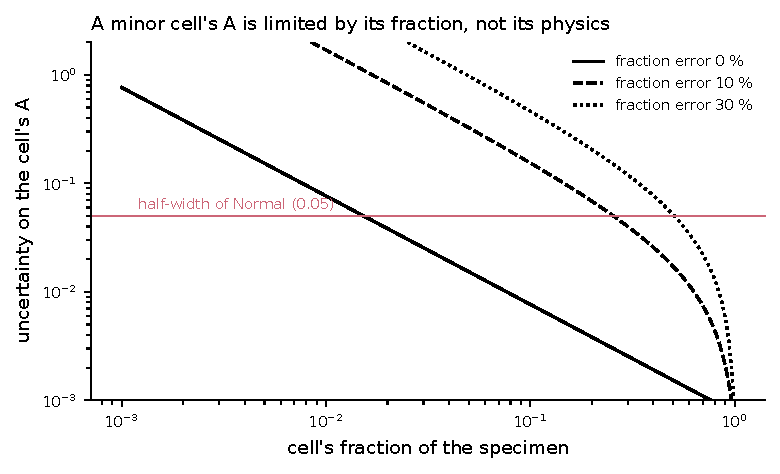
\includegraphics[width=0.8\textwidth]{figures/part4/fig_fraction_precision.pdf}
\caption{Uncertainty on a cell's $A$ against its fraction of the specimen, for 2,000 identity loci, array noise 0.02 in $\beta$, the immune floor,
and a background that differs from the cell by 0.1 in $\beta$ at those loci. The three curves assume a relative error of 0, 10 and 30~\% in the other
cells' fractions. \calc}
\label{fig:fracprec}
\end{figure}

\begin{rulebox}
Fraction is the detection gate. Above the gate a cell is read; where the uncertainty set by its fraction exceeds the half-width of Normal, the reading
is printed and the tier word is withheld, with one line saying why: not enough of this cell to score it confidently.
\end{rulebox}

\section{A second opinion}

Cosmology never trusted one separation method. The commissioned chain keeps a second, blind solver (an internal-linear-combination style method) whose composition
is shown beside the primary's as a cross-check on the Safeguards tab; the v2 reader does not yet carry one. It never replaces the primary and never changes a reading; a disagreement between
the two is flagged.

\section{Cells that should not be there}

A cell that is not normally in the specimen, epithelium or neurons in blood, is found by a joint fit in which blood cells and all non-blood templates are
solved together, so a foreign cell competes for mass on equal terms. An earlier design fitted blood first and looked for foreign cells in the residual; it
absorbed real foreign material into blood. A non-blood cell in whole blood is scored only when it is detected. \measured
